\section{Grundlagen}
\label{sec:grundlagen}

Folgendes Kapitel beschreibt die Robotik und die benötige Einordnung der Arbeit in diese.
Hierfür wird die Robotik oberflächlich definiert, eingeteilt und die relevanten Teilbereiche dieser genauer betrachtet.
Da diese Arbeit sich mit einem \gls{go1} beschäftigt, wird dieser klassifiziert und in die Bereiche der Forschung, Industrie und weiterer Nutzung eingeordnet.
Zum weiteren Verständnis des Ziels der Arbeit - der Analyse und Integration des \gls{go1} in ein bestehendes Ökosystem -
wird der aktuelle Stand der Forschung genauer betrachtet.
Relevant sind hier besonders die bereits erarbeiteten Erkenntnisse der Nutzung gleicher oder ähnlicher Roboter, als auch
die Einbindung anderer Modelle in bestehende Ökosysteme.
Hierfür soll nicht nur die Forschung allein betrachtet werden, sondern auch die Arbeit privater Unternehmen und Entwickler.
Mit dem Wissen der korrekten Einordnung des \gls{go1} und dem Forschungsstand zu verwandten Themen sollen die Herausforderungen dieser
Arbeit hervorgehoben werden, sodass im späteren Verlauf die Erarbeitungen auf die bekannten Probleme verweisen können.

\subsection{Robotik}
\label{subsec:robotik}

Die Robotik befasst sich mit dem Wissensgebiet rund um \emph{Roboter}.
Der Begriff \emph{Roboter} stammt vom tschechischen Wort \emph{robota}, was so viel wie \emph{Frondienst} oder \emph{Zwangsdienst} bedeutet.
So treffend diese Übersetzung auf die heutige Nutzung des Wortes ist, so vage ist diese Beschreibung auch.
Ähnlich unklar sind auch die anerkannten Definitionen des Wortes \emph{Roboter}.
Eine gängige Definition im deutschsprachigen Raum ist die des \gls{vdi}:

\begin{quote}
    Industrieroboter sind universell einsetzbare Bewegungsautomaten mit mehreren Achsen,
    deren Bewegungen hinsichtlich Bewegungsfolge und Wegen bzw.
    Winkeln frei (d.h, ohne mechanischen Eingriff) programmierbar und ggf.~sensorgeführt sind\footcite{vdi_2860}.
\end{quote}

Auch wenn die \gls{vdi}-Richtlinie mittlerweile zurückgezogen wurde, wird die Definition aufgrund ihrer treffenden Eingrenzung
des Begriffes noch häufig zitiert.

Die umstrittene Definition des Begriffs \emph{Roboter} zieht eine ebenso unklare Einteilung des Wissensfeldes der \emph{Robotik} mit sich.
Hält man sich jedoch an die Definition des \gls{vdi}, so lassen sich Roboter in zwei Kategorien einteilen, Industrieroboter und Serviceroboter.
Abbildung~\ref{fig:industrie_vs_service}\footcite{statista_robotics_market} zeigt die beiden Klassifizierungen und deren Eigenschaften im Überblick.

\begin{figure}[h]
    \frame{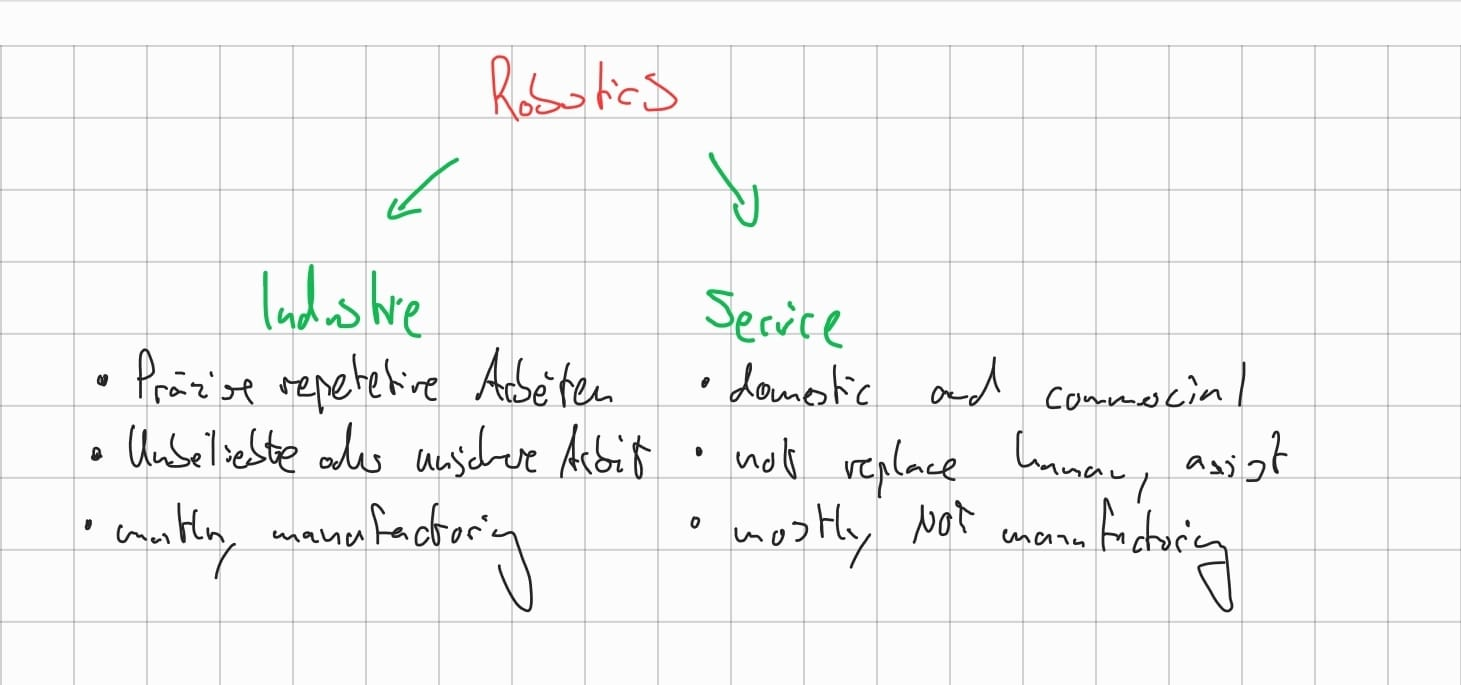
\includegraphics[width=\linewidth]{img/architektur/industrie_vs_service}}
    \caption{Vergleich zwischen Industrie- und Servicerobotern}\label{fig:industrie_vs_service}
\end{figure}

\subsubsection{Industrieroboter}

Industrieroboter sind Roboter, die im industriellen Umfeld eingesetzt werden den Mensch meist in nicht sicheren,
nicht rentablen oder nicht begehrenswerten - repetitiven - Arbeiten ersetzen.
Sie sind aufgrund ihrer hohen Spezialisierung an den Einsatzzweck großenteils stationär.
Der Vorteil industriell eingesetzter Roboter ist die hohe Effizienz und Genauigkeit der Arbeiten und die Anpassbarkeit an
den Einsatzzweck.
Als Nachteil ergibt sich hieraus der hohe Aufwand der Implementierung, da ein hoch spezialisierter Roboter für jeden
Einsatzzweck neu geschaffen werden muss.
Einsatzzwecke von Industrierobotern sind unter anderen das Schweißen, Lackieren, Montieren und die Materialhandhabung in
Produktionsumgebungen.

Die Limitierung des Einsatzes und die strikte Einteilung zu industriellen Einsätzen lässt schlussfolgern, dass der \gls{go1}
nicht in die Klasse der Industrieroboter eingegliedert werden kann.
Stattdessen kann man ihn in der in dieser Arbeit verwendeten, einfachen Unterteilung den Servicerobotern zuteilen.

\subsubsection{Serviceroboter}

Serviceroboter unterscheiden sich im Kern von Industrierobotern in der Annahme, dass sie Menschen in ihrem Einsatzzweck nicht ersetzen,
sondern unterstützen oder von Menschen unterstützt werden.
Der Begriff \emph{Serviceroboter} ist absichtlich weit gefasst und schließt im Umfang dieser Arbeit lediglich industrielle
Roboter, so wie sie im vorigen Paragrafen beschrieben werden, aus.
Bei Serviceroboter lässt sich grundsätzlich noch zwischen kommerziell eingesetzten und konsumorientierten Robotern unterscheiden\footcite{statista_robotics_market}.

Serviceroboter sind in der Regel nicht stationär, da sie in ihren Einsatzmöglichkeiten deutlich flexibler sind, als Industrieroboter.
Aus dem Vorteil der Flexibilität lässt sich ebenfalls der Nachteil der Komplexität ableiten.
Das weitere Einsatzfeld der Serviceroboter steigert in der Regel den Aufwand der Entwicklung, steigert aber ebenfalls
den Ertrag des Roboters, finanziell auch den \gls{roi}.

Möchte man die Klasse der Serviceroboter weiter untergliedern, so sind unter anderen folgende Untergliederungen denkbar:

\begin{itemize}
    \item Spielzeugroboter
    \item Erkundungsroboter
    \item Militär-/ Kampfroboter
    \item Assistenzroboter
\end{itemize}

Zu Vermerken ist, dass die simple Klassifizierung der Roboter in lediglich zwei Klassen der Industrieroboter und der Serviceroboter
gewählt wurde, um die Einsatzzwecke des \gls{go1} in dieser Arbeit nicht einzuschränken.
Wie bereits erarbeitet kann man den \gls{go1} vielseitig einsetzen, jedoch ist er nicht geeignet, Menschen in seinen Einsatzgebieten
vollständig zu ersetzen, noch ist er strikt auf industrielle Zwecke beschränkt.
Eine Zuteilung zu industriellen Robotern ist somit nicht möglich.
Eine genauere Klassifizierung innerhalb der Klasse der Serviceroboter ist zwar möglich, jedoch vom finalen Einsatzzweck des
Quadruped Roboters abhängig.
Mögliche Einsatzzwecke werden später in dieser Arbeit erörtert.

\subsubsection{Cobots}

Ein weiterer passender Begriff, der der Klassifizierung des \gls{go1} als Serviceroboter nicht widerspricht, ist \emph{Cobot}
\emph{Cobot} setzt sich aus dem Englischen Wort \emph{collaborate} - (zusammenarbeiten, kollaborieren) und dem Wort \emph{Roboter}
zusammen.
Einige Merkmale sind:\footcite{statista_robotics_market}

\begin{itemize}
    \item Kollaborativ und sicher, im Gegensatz zu stationär und abgesichert
    \item Interaktiv und adaptiv zur Umgebung
    \item Einfache Inbetriebnahme durch vorausschauende Entwicklung
    \item Flexible Einsatzzwecke
    \item Schnelleres \gls{roi}
\end{itemize}

Durch seine flexiblen Fortbewegungsmöglichkeiten und der hohen Anzahl an Sensorik und Erweiterungsmöglichkeiten des \gls{go1}
sowie der zur Kollaboration einladenden Vorrichtungen wie den Mikrofonen und Lautsprechern\footnote{Siehe Kapitel~\ref{subsubsec:hardware_sensorik}}
lässt sich der \gls{go1} neben der Klassifizierung als Serviceroboter ebenfalls als \emph{Cobot} bezeichnen.
Der kollaborative Aspekt und die Unterstützung des Menschen statt der Ersetzung dessen wird im Laufe der Arbeit weiter erörtert.
\todo{Herleitung Quadruped}

\subsection{Stand der Forschung}
\label{subsec:stand-der-forschung}

Im Bereich der Quadruped Roboter ist bereits viel erforscht worden.
Besonders im Fokus der Arbeiten sind in der Regel die Steuerung der Motoren zur Fortbewegung, die autonome Navigation
der Roboter in unbekanntem Umfeld und das Testen der Einsatzmöglichkeiten der vierbeinigen Roboter.
Diese Arbeit hingegen beschäftigt sich mit der Integration des Roboters in ein Hochschulökosystem, welche die möglichen Einsatzzwecke
nicht vorwegnimmt.
Ziel dieser Arbeit ist es, Einsatzmöglichkeiten zu erarbeiten und die nötigen Anpassungen am Model \gls{go1} vorzunehmen,
um diese zu ermöglichen.
Deshalb werden im folgenden nur kurz allgemein interessante Forschungen an Quadruped Robotern gezeigt, wonach
allgemeine Forschungen zur Einbindung und Nutzung von Servicerobotern dargestellt werden.
Zuletzt sollen noch Arbeiten speziell zum Modell \gls{go1} gezeigt werden.
Diese werden nicht zwingend akademischen Ursprungs sein und sollen dem Leser der Arbeit einen Überblick über die vorhandenen
Ressourcen zum Modell \gls{go1} bieten.

\subsubsection{Quadruped Roboter}

\subsubsection{Integration von Robotern}

\subsubsection{Unitree Go1 Ressourcen}


\subsection{Herausforderungen}
\label{subsec:herausforderungen}


%\subsection{Begriffe}
\label{subsec:begriffe}

Zur Einführung in die tatsächlichen Inhalte der Arbeit sollen die Begriffe \emph{Robotik} beziehungsweise \emph{Roboter} und \emph{\gls{ki}} genauer erläutert werden.
Durch die Erklärung und Abgrenzung der Begriffe und ihrer Relevanz für diese Arbeit wird im Anschluss noch die Verbindung der Bereiche erläutert.

\subsubsection{Robotik}
Wie der Titel dieser Arbeit \enquote{\mytitle} erkennen lässt, handelt diese Arbeit hauptsächlich vom Umgang und dem sinnvollen Einsatz eines Roboters.
Das Fachgebiet, welches sich mit Robotern beschäftigt, bezeichnet sich trivialerweise mit dem Begriff \emph{Robotik}.

Die Definition des Wortes \emph{Roboter} ist hingegen nicht so trivial.
So beziehen sich viele wissenschaftliche Definitionen oftmals genauer auf Industrieroboter, welche den einfachen Zweck der Entlastung menschlicher Arbeitskräfte haben.
In der Gesellschaft werden Roboter jedoch oftmals als Maschinen verstanden, die dem Menschen oder anderen bereits bekannten Kreaturen sehr ähnlich sind.\footcite{grundlagen_der_robotik}
Allgemein lässt sich das Wort \emph{Roboter} vermutlich mit folgender Definition weit fassend beschreiben:

\begin{quote}
    [...] Automat, der ferngesteuert oder nach Sensorsignalen bzw.\ einprogrammierten Befehlsfolgen anstelle eines Menschen bestimmte mechanische Tätigkeiten verrichtet\footcite{duden_roboter}
\end{quote}

% Etwas Geschichte?

Geschichtlich ordnen sich die ersten Ideen, die heute mindestens entfernt der Robotik zuzuordnen sind, in die Zeit der Antike ein.
Die Idee der Maschine, welche dem Menschen einfache Arbeiten abnehmen kann oder derer, die von menschlicher Hand gefertigt den Menschen gleich ist, hat seit dem über die gesamte vergangene Zeit die Kreativen der Welt begeistert.
Von automatisierten Maschinen aus den Skizzenbüchern des \emph{Da Vinci} bis hin zu den ersten Mensch-ähnlichen Maschinen der Firma \emph{Honda} in den späten \num{1990}-ern.\footcite{grundlagen_der_robotik}
% Abschluss
Der Vielfalt der Robotik entgegen wird sich diese Arbeit außerhalb der Grundlagenbereiche ausschließlich mit vierbeinigen Robotern auseinandersetzen, welche oftmals durch ihre Ähnlichkeit mit Hunden herausstechen.

\todo{Einordnung relevanz allgemeiner Robotik für arbeit}
\todo{relevant?}

\subsubsection{Künstliche Intelligenz}
% Was ist es allgemein? Kurz
% Wie wird es in Verbindung mit Robotik genutzt?


\subsubsection{Webkommunikation}
% Was ist allgemein relevant?
% Warum hier relevant
% TCP. Portfreigaben, Netzwerke


\subsubsection{Internet of Things}
% relevant hier? oder bei MQTT?
% Protokolle anbringen?


\subsubsection{Einordnung}

% Wie sind Roboter und KI in dieser Arbeit vernetzt, worin kann man sie in ihren Gebieten einordnen? Humanoid, etc.
% Robotik, was relevant? BMS, Steuerung per Fernsteuerung, Aufnahme der Daten (Video, Audio, Sensoren)
% ML - Wie könnte es allgemein hier relevant sein? -> Auslagerung auf Server wg rechenleistung
% IoT - Edgedevice, kommuniziert mit anderen Geräten, ist aber auch broker an sich
%\subsection{Herausforderungen}
\label{subsec:herausforderungen}

\subsubsection{Netzwerk, Latenz, Resilienz...}
%\subsection{Stand der Forschung}
\label{subsec:stand-der-forschung}

